% L2ODLL: Dual Lagrangian Learning.
%
% A proxy f_theta predicts the dual variables y-hat of the predicted block from
% the parameters p; the prediction is projected onto the dual cone, y-bar =
% Pi_{C*}(y-hat); the remaining duals z are completed by the completion problem
% (3), in closed form for bounded variables (4) and strictly convex quadratic
% objectives (6); the completed dual objective Phi(y-bar, p) is a dual bound
% and, maximized in expectation (7), the self-supervised training loss.
% Notation and equation numbers follow docs/src/theory.md (MOI sign convention).
%
% Build: make -C docs/src/assets/diagrams/src
%   pdflatex -jobname=l2odll--dual-completion dll.tex          -> wide layout
%   pdflatex -jobname=l2odll--dual-completion-compact dll.tex  -> narrow layout
\documentclass[tikz,border=4pt]{standalone}
% Shared style of the LearningToOptimize diagrams: the palette, lane frames, cards,
% chips and glyphs of the paper-style TikZ figures (the same visual system as the
% PortfolioOpt.jl and DecisionRules.jl figures). Each figure \input's this file.
\usepackage{amsmath,amssymb,bm}
\usepackage[T1]{fontenc}
\usepackage[scaled=0.92]{helvet}
\renewcommand{\familydefault}{\sfdefault}
\usetikzlibrary{arrows.meta,shapes.geometric,shapes.symbols,calc,positioning,decorations.pathreplacing}

\definecolor{dTeal}{HTML}{1A9AA0}
\definecolor{dTealLine}{HTML}{3FB3B8}
\definecolor{dNavy}{HTML}{3F4C8C}
\definecolor{dInk}{HTML}{1E2235}
\definecolor{dRed}{HTML}{E4573D}
\definecolor{dCoral}{HTML}{E2765A}
\definecolor{dOrange}{HTML}{F4A93B}
\definecolor{dPeach}{HTML}{FBD9AC}
\definecolor{dPanel}{HTML}{EEF0F2}
\definecolor{dGray}{HTML}{8A90A0}
\definecolor{dNode}{HTML}{14A3A8}
\definecolor{dShadow}{HTML}{D5DAE3}

% \ifcompact is true when the job name ends in "-compact" (narrow layout).
\newif\ifcompact
\ifnum\pdfmatch{-compact$}{\jobname}=1 \compacttrue\fi

\tikzset{
  >={Stealth[length=5pt,width=4pt]},
  every node/.style={text=dInk},
  title/.style={anchor=west,font=\small,inner sep=0pt},
  head/.style={font=\small\bfseries,text=dNavy},
  note/.style={font=\itshape\footnotesize,text=dNavy},
  dnote/.style={font=\itshape\footnotesize,text=dCoral},
  code/.style={font=\ttfamily\footnotesize,text=dNavy},
  store/.style={cylinder,shape border rotate=90,aspect=0.28,fill=dPeach,draw=dOrange,
                line width=0.7pt,minimum width=0.95cm,minimum height=1.2cm,font=\normalsize},
  dia/.style={diamond,fill=dOrange,draw=none,minimum size=0.9cm,inner sep=0pt,aspect=1,
              font=\normalsize},
  lnode/.style={circle,fill=dRed,draw=none,minimum size=0.66cm,inner sep=1pt,
                text=white,font=\normalsize},
  card/.style={rectangle,rounded corners=4pt,fill=white,draw=dShadow,line width=0.6pt},
  sheet/.style={rectangle,rounded corners=3pt,fill=dPanel,draw=dShadow,line width=0.6pt},
  chip/.style={rectangle,rounded corners=3pt,fill=dPanel,draw=none,font=\small,
               inner xsep=4pt,inner ysep=3pt},
  ochip/.style={chip,fill=white,draw=dGray,dashed,line width=0.6pt},
  pchip/.style={chip,fill=white,draw=dGray!70,dashed,line width=0.5pt,text=dGray},
  fwd/.style={->,dTealLine,line width=0.8pt},
  tgt/.style={->,dOrange,line width=0.9pt},
  dual/.style={->,dCoral,dashed,line width=0.9pt},
  dep/.style={->,dTealLine,line width=0.8pt},
  pdep/.style={->,dGray,dashed,line width=0.7pt},
  nn/.style={circle,minimum size=0.26cm,inner sep=0pt,draw=dInk!70,line width=0.35pt},
}

% Lane frame in the paper style: two shadow copies behind a teal rounded frame.
\newcommand{\lane}[4]{% #1 x0, #2 y0, #3 x1, #4 y1
  \foreach \o/\c in {0.16/dShadow!60,0.08/dShadow}
    \draw[\c,fill=white,rounded corners=5pt,line width=0.6pt]
      (#1+\o,#2-\o) rectangle (#3+\o,#4-\o);
  \draw[dTealLine,fill=white,rounded corners=5pt,line width=0.9pt] (#1,#2) rectangle (#3,#4);}

% Plain card frame (no shadow copies), for problems and losses.
\newcommand{\cardbox}[4]{\draw[dShadow,fill=white,rounded corners=4pt,line width=0.6pt] (#1,#2) rectangle (#3,#4);}

% Network glyph on one sheet. #1 = centre, #2 = name prefix, #3 = number of stacked
% sheets behind (0, 1 or 2).
\newcommand{\net}[3]{%
  \begin{scope}[shift={(#1)}]
    \ifnum#3>1 \node[sheet,minimum width=1.9cm,minimum height=1.8cm] at (0.30,0.22) {};\fi
    \ifnum#3>0 \node[sheet,minimum width=1.9cm,minimum height=1.8cm] at (0.15,0.11) {};\fi
    \node[sheet,minimum width=1.9cm,minimum height=1.8cm,fill=white] (#2sheet) at (0,0) {};
    \foreach \y [count=\i] in {0.36,0,-0.36} \node[nn,fill=dGray!45] (#2in\i) at (-0.64,\y) {};
    \foreach \y [count=\i] in {0.58,0.29,0,-0.29,-0.58} \node[nn,fill=dNode] (#2ha\i) at (-0.21,\y) {};
    \foreach \y [count=\i] in {0.44,0.15,-0.15,-0.44} \node[nn,fill=dNode] (#2hb\i) at (0.21,\y) {};
    \node[nn,fill=dOrange] (#2out) at (0.64,0) {};
    \foreach \a in {1,...,3} \foreach \b in {1,...,5} \draw[dGray!60,line width=0.2pt] (#2in\a) -- (#2ha\b);
    \foreach \a in {1,...,5} \foreach \b in {1,...,4} \draw[dGray!60,line width=0.2pt] (#2ha\a) -- (#2hb\b);
    \foreach \a in {1,...,4} \draw[dGray!60,line width=0.2pt] (#2hb\a) -- (#2out);
  \end{scope}}

% Jacobian mask glyph: an n x d grid with a few entries selected. #1 = centre.
\newcommand{\maskgrid}[1]{%
  \begin{scope}[shift={(#1)}]
    \foreach \i in {0,...,4} \foreach \j in {0,...,3}
      \draw[dShadow,fill=white,line width=0.4pt] (\j*0.2-0.4,-\i*0.2+0.5) rectangle ++(0.2,-0.2);
    \foreach \i/\j in {0/1,1/3,2/0,3/2,4/1}
      \draw[dOrange,fill=dOrange,line width=0.4pt] (\j*0.2-0.4,-\i*0.2+0.5) rectangle ++(0.2,-0.2);
  \end{scope}}

% Code names inside italic notes stay upright.
\newcommand{\cmd}[1]{{\upshape\ttfamily #1}}

% Software-architecture helpers: package cards, type chips and chip rows.
\tikzset{
  pkg/.style={rectangle,rounded corners=4pt,fill=white,draw=dShadow,line width=0.6pt,
              align=center,inner xsep=5pt,inner ysep=4pt,font=\footnotesize},
  pkgcore/.style={pkg,draw=dTealLine,line width=0.9pt},
  pkgplan/.style={pkg,draw=dGray,dashed,text=dGray},
  tchip/.style={chip,font=\ttfamily\footnotesize,inner xsep=3pt,inner ysep=2.5pt},
  tplan/.style={tchip,fill=white,draw=dGray,dashed,line width=0.5pt,text=dGray},
  absname/.style={anchor=west,font=\ttfamily\footnotesize,text=dNavy,inner sep=1pt},
}
% \chiprow{x}{y}{style}{A,B,C}: chips left to right from (x,y), anchored west.
\newcommand{\chiprow}[4]{%
  \coordinate (cr@next) at (#1,#2);
  \foreach \t in {#4} {%
    \node[#3,anchor=west] (cr@last) at (cr@next) {\t};
    \coordinate (cr@next) at ($(cr@last.east)+(0.12,0)$);}}


\newcommand{\completion}{%
  $\begin{aligned}
    \Phi(\bar y,p)=\max_{z}\;\; & -h(p)^\top z-b(p)^\top\bar y\\[1pt]
    \text{s.t.}\;\; & H^\top z=c(p)-A^\top\bar y\\[1pt]
    & z\in\mathcal{K}^*
  \end{aligned}$}
\newcommand{\quadratic}{strictly convex quadratic (6):\; $w=Q^{-1}\big(A^\top\bar y-c(p)\big)$}
\newcommand{\training}{$\max_\theta\;\mathbb{E}_{p}\big[\Phi\big(\Pi_{\mathcal{C}^*}(f_\theta(p)),\,p\big)\big]$}

\begin{document}
\ifcompact
% ============================ narrow (phone) layout ============================
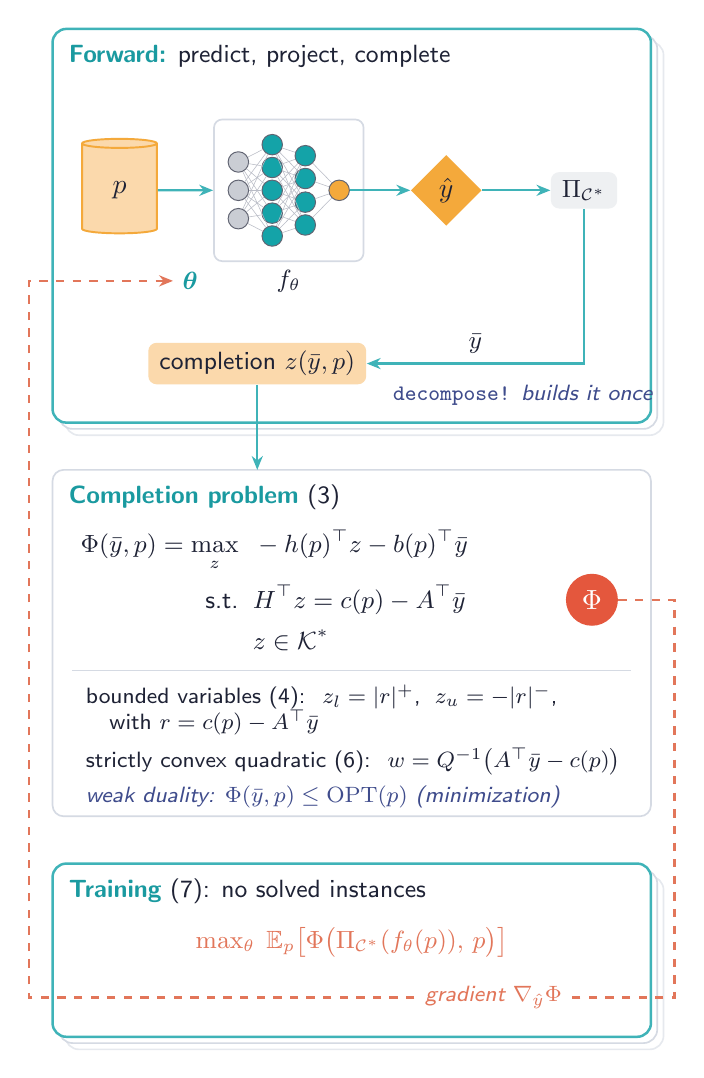
\begin{tikzpicture}
  % ---- forward ----
  \lane{0}{7.6}{7.6}{12.6}
  \node[title] at (0.2,12.25) {\textcolor{dTeal}{\bfseries Forward:} predict, project, complete};
  \node[store] (p) at (0.85,10.55) {$p$};
  \net{3.0,10.55}{px}{0}
  \node[font=\small] at (3.0,9.4) {$f_\theta$};
  \node[font=\small\bfseries,text=dTeal] (th) at (1.75,9.4) {$\bm\theta$};
  \draw[fwd] (p.east) -- (pxsheet.west);
  \node[dia] (yh) at (5.0,10.55) {$\hat y$};
  \draw[fwd] (pxout.east) -- (yh.west);
  \node[chip] (pi) at (6.75,10.55) {$\Pi_{\mathcal{C}^*}$};
  \draw[fwd] (yh.east) -- (pi.west);
  \node[chip,fill=dPeach] (cp) at (2.6,8.35) {completion $z(\bar y,p)$};
  \draw[fwd] (pi.south) |- node[pos=0.75,above,font=\small] {$\bar y$} (cp.east);
  \node[note,anchor=west] at (4.2,7.95) {\cmd{decompose!} builds it once};
  % ---- completion problem ----
  \cardbox{0}{2.6}{7.6}{7.0}
  \draw[fwd] (cp.south) -- (2.6,7.0);
  \node[title] at (0.2,6.65) {\textcolor{dTeal}{\bfseries Completion problem} (3)};
  \node[anchor=north west,font=\small,inner sep=0pt] at (0.35,6.25) {\completion};
  \node[lnode] (phi) at (6.85,5.35) {$\Phi$};
  \draw[dShadow,line width=0.6pt] (0.25,4.45) -- (7.35,4.45);
  \node[font=\footnotesize,anchor=west,align=left] at (0.3,3.95) {bounded variables (4):\; $z_l=\lvert r\rvert^+$,\; $z_u=-\lvert r\rvert^-$,\\\hspace*{1em}with $r=c(p)-A^\top\bar y$};
  \node[font=\footnotesize,anchor=west] at (0.3,3.3) {\quadratic};
  \node[note,anchor=west] at (0.3,2.85) {weak duality: $\Phi(\bar y,p)\le\mathrm{OPT}(p)$ (minimization)};
  % ---- training ----
  \lane{0}{-0.2}{7.6}{2.0}
  \node[title] at (0.2,1.65) {\textcolor{dTeal}{\bfseries Training} (7): no solved instances};
  \node[font=\small,text=dCoral] (tr) at (3.8,1.0) {\training};
  \draw[dual] (phi.east) -- (7.9,5.35) -- (7.9,0.3) -- (-0.3,0.3) -- (-0.3,9.4) -- (th.west);
  \node[dnote,fill=white,inner sep=1pt] at (5.6,0.3) {gradient $\nabla_{\hat y}\Phi$};
\end{tikzpicture}
\else
% =============================== wide layout ===================================
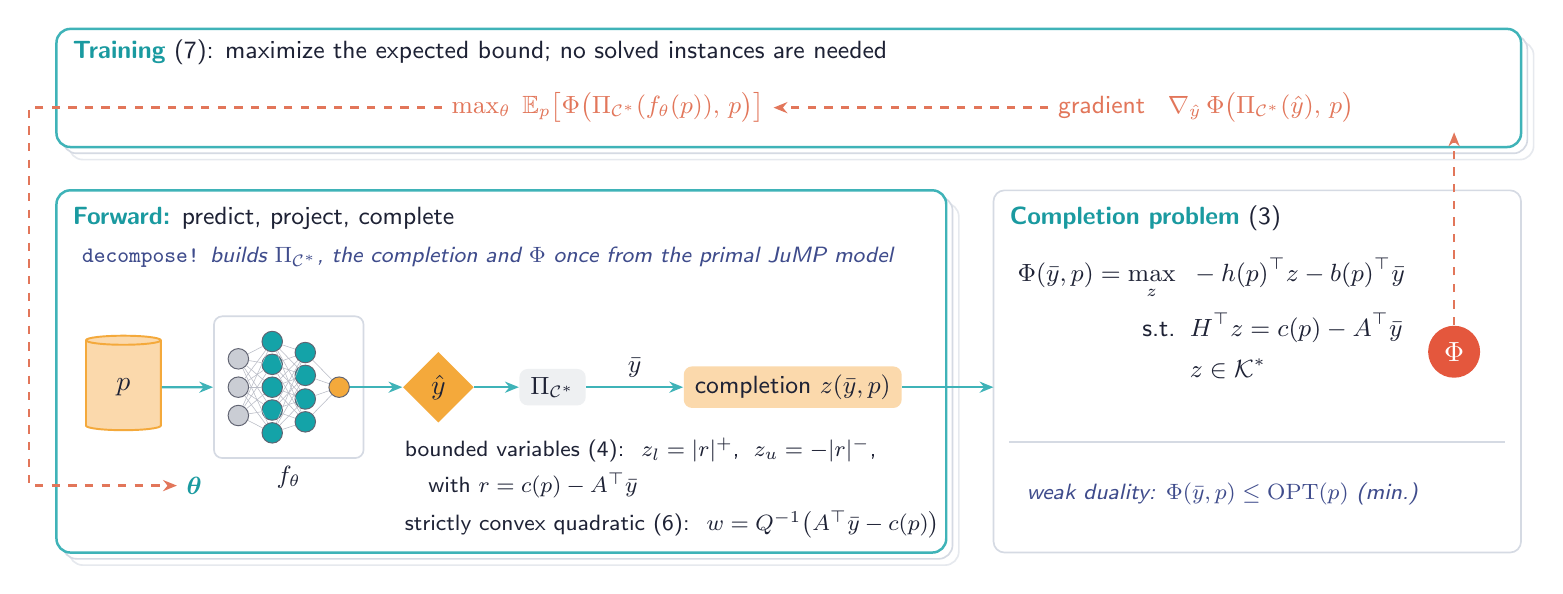
\begin{tikzpicture}
  % ---- training band (top) ----
  \lane{0}{5.15}{18.6}{6.65}
  \node[title] at (0.2,6.35) {\textcolor{dTeal}{\bfseries Training} (7): \textcolor{dInk}{maximize the expected bound; no solved instances are needed}};
  \node[font=\small,text=dCoral] (tr) at (7.0,5.65) {\training};
  \node[font=\small,text=dCoral] (gr) at (14.6,5.65) {gradient\;\; $\nabla_{\hat y}\,\Phi\big(\Pi_{\mathcal{C}^*}(\hat y),\,p\big)$};
  \draw[dual] (gr.west) -- (tr.east);

  % ---- forward (bottom left) ----
  \lane{0}{0}{11.3}{4.6}
  \node[title] at (0.2,4.25) {\textcolor{dTeal}{\bfseries Forward:} \textcolor{dInk}{predict, project, complete}};
  \node[note,anchor=west] at (0.2,3.75) {\cmd{decompose!} builds $\Pi_{\mathcal{C}^*}$, the completion and $\Phi$ once from the primal JuMP model};
  \node[store] (p) at (0.85,2.1) {$p$};
  \net{2.95,2.1}{px}{0}
  \node[font=\small] at (2.95,0.95) {$f_\theta$};
  \node[font=\small\bfseries,text=dTeal] (th) at (1.75,0.85) {$\bm\theta$};
  \draw[fwd] (p.east) -- (pxsheet.west);
  \node[dia] (yh) at (4.85,2.1) {$\hat y$};
  \draw[fwd] (pxout.east) -- (yh.west);
  \node[chip] (pi) at (6.3,2.1) {$\Pi_{\mathcal{C}^*}$};
  \draw[fwd] (yh.east) -- (pi.west);
  \node[chip,fill=dPeach] (cp) at (9.35,2.1) {completion $z(\bar y,p)$};
  \draw[fwd] (pi.east) -- node[above,font=\small] {$\bar y$} (cp.west);
  \node[font=\footnotesize,anchor=west] at (4.3,1.3) {bounded variables (4):\; $z_l=\lvert r\rvert^+$,\; $z_u=-\lvert r\rvert^-$,};
  \node[font=\footnotesize,anchor=west] at (4.3,0.85) {\hspace*{1em}with $r=c(p)-A^\top\bar y$};
  \node[font=\footnotesize,anchor=west] at (4.3,0.35) {\quadratic};

  % ---- completion problem (bottom right) ----
  \cardbox{11.9}{0}{18.6}{4.6}
  \node[title] at (12.1,4.25) {\textcolor{dTeal}{\bfseries Completion problem} (3)};
  \node[anchor=north west,font=\small,inner sep=0pt] at (12.2,3.75) {\completion};
  \draw[dShadow,line width=0.6pt] (12.1,1.4) -- (18.4,1.4);
  \node[note,anchor=west] at (12.2,0.75) {weak duality: $\Phi(\bar y,p)\le\mathrm{OPT}(p)$ (min.)};
  \draw[fwd] (cp.east) -- (11.9,2.1);
  \node[lnode] (phi) at (17.75,2.55) {$\Phi$};
  \draw[dual] (phi.north) -- (gr.south -| phi.north);
  \draw[dual] (tr.west) -| (-0.35,0.85) -- (th.west);
\end{tikzpicture}
\fi
\end{document}
